%
%  Thesis Vorlage für die Hochschule Heilbronn
%
%  Created by Prof. Dr. Detlef Stern on 2010-08-14.
%  Updated by Valentin Weber on 2020-10-05.
%  Copyright (c) 2020 . All rights reserved.
%
\documentclass[12pt,toc=bib,toc=listof]{scrreprt}
\usepackage[ngerman]{babel} 
\usepackage[utf8]{inputenc}
\usepackage[T1]{fontenc}
\usepackage{lmodern}
\usepackage{setspace}
\usepackage{geometry}

\usepackage{hyperref}
\hypersetup{
  ,colorlinks=true
  ,linkcolor=blue
  ,citecolor=blue
  ,filecolor=blue
  ,urlcolor=blue
  }

% Fachbezogene Werte (müssen aktualisiert werden)
\newcommand{\hhnsubject}{COMPUTER AND ROBOTVISION}
\newcommand{\hhnsubjectnum}{PRÜFUNGSNUMMER: 135031}
\newcommand{\hhnlecturer}{PROF. DR. DIETER MAIER}

% Vom Studierenden zu aendernde Werte
\newcommand{\reprttopic}{BRIEFMARKENERKENNUNG}
\newcommand{\reprtstudentname}{GEORG JAHN, MARTIN HAAG}
\newcommand{\reprtstudentid}{195XXX, 194980}
\urldef{\reprtstudentmail}\url{gjahn@stud.hs-heilbronn.de ,mahaag@stud.hs-heilbronn.de}

\usepackage{ifpdf}
\ifpdf
\usepackage[pdftex]{graphicx}
\else
\usepackage{graphicx}
\fi

\usepackage[headsepline]{scrlayer-scrpage}
\pagestyle{scrheadings}
\clearscrheadfoot
\ihead{\hhnsubject: \reprttopic}
\ohead{\pagemark}
\renewcommand*{\chapterpagestyle}{scrheadings}
\renewcommand*{\chapterheadstartvskip}{}

%meine adds
\usepackage[belowskip=-15pt,aboveskip=0pt]{caption}
\renewcaptionname{ngerman}\figurename{Abb.}	
\usepackage{caption}
\captionsetup{format=plain}
\usepackage[section]{placeins} 

% Deckblatt Definitionen (begin)
\titlehead{\flushright
\includegraphics{./bilder/hhn.png}}
\subject{{\hhnsubject{} (\hhnsubjectnum{})}}
\title{\reprttopic}
\author{\reprtstudentname\footnote{\reprtstudentid, \reprtstudentmail}}
%% Datum nie auf einen festen Wert setzen
\publishers{Eingereicht bei \hhnlecturer}
% Deckblatt Definitionen (end)

\begin{document}
\renewcommand*{\figurename}{Abb.}
\pagenumbering{Roman} 
\selectlanguage{ngerman}
\maketitle
\newgeometry{left=30mm, top=25mm, right=15mm, bottom=25mm}

\tableofcontents

\addchap{Abkürzungs- Fremdwort und Fachbegriffsverzeichnis} % (fold)
\label{sec:abkuerzungsverzeichnis}

\begin{description}
  \item[NN:] neuronales Netz(-werk)
  \item[CNN:] convolutional neuronal network
  \item[Transfer Learning:] Technik, bei der ein bestehendes NN auf ein anders, vergleichbares Problem angewandt wird und dadurch nur wenig trainiert werden muss  
  \item[RGB-Bild:] Bild mit den Farbkanälen in dieser Reihenfolge
  \item[Otsu-Methode:] Methode zur Festlegung eines Schwellwertes zur Binarisierung auf Grundlage des Histogrammes
  \item[morphologischer Filter:] Filter, die im Stande sind, Strukturen von Bildern gezielt zu beeinflussen \cite{digi_bv}
  \item[PAP: ] Programmablaufplan
  \item[Supervised Learning: ] Lernvorgang anhand eines Datensatzes, bei dem das Musterergebnis bekannt ist
  \item[Relu6: ] Rectified Linear Unit, eine nicht lineare Aktivierungsfunktion 
  \item[Adam-Optimizer:] eine Methode zur iterativen Anpassung der Gewichte in einem NN
  \item[Epoche:] ein ganzer Trainingsdurchgang durch alle Trainingsdaten 
  \item[Forwardpass:] Berechnung eines Outputs eines NN anhand eines Inputs
  \item[Data Augmentation:] Erweiterung eines Datensatzes durch Abänderung bestehender Daten
   
\end{description}

% chapter abkuerzungsverzeichnis (end)

\onehalfspacing


% chapter management_summary (end)
\newpage
\pagenumbering{arabic}

% report (begin)
\chapter{Einleitung} % (fold)
\label{sec:einleitung}

\section{Motivation} % (fold)
\label{sec:motivation}
Bildverarbeitung ist kein neues Feld der Forschung mehr und auch neuronale Netzwerke sind bereits seit vielen Jahren Subjekt von ständiger Weiterentwicklung. Da diese beiden Fachgebiete durchaus gut miteinander harmonieren, haben wir uns entschieden, in unserem Projekt eine Aufgabe, die beides benötigt, zu bearbeiten. Im Rahmen unseres CRV Projektes haben wir deshalb die Unterscheidung von Briefmarken in gestempelte und ungestempelte automatisiert mithilfe einer künstlichen Intelligenz durchgeführt. Wenn auch unsere Arbeit sehr unwahrscheinlich kommerzielle Anwendung findet, ist es doch geeignet, um an einem Tag der offenen Tür oder einem \dq studieren probieren\dq\ Event demonstriert zu werden.

% section motivation (end)

\section{Ziel der Arbeit} % (fold)
\label{sec:ziel_der_arbeit}
Das Ziel der Arbeit war es, mithilfe eines Teils klassischer Bildverarbeitung und eines neuronalen Netzwerkes (NN) Bilder von gestempelten von Bildern mit ungestempelten Briefmarken zu unterscheiden.Ursprünglich war der Plan, mit Bildern von ganzen Briefen zu arbeiten. Der Vorteil bei diesem Ansatz wäre, dass die Überlappung des Stempels über Briefmarke und Brief es wohl für das Netzwerk einfacher gemacht hätte, die Klassen gestempelt/nicht gestempelt zu unterscheiden. Aufgrund von Datenschutzgesetzen waren wir jedoch nicht in der Lage, einen ausreichend großen Datensatz zusammen zu tragen. Deshalb haben wir uns entschieden, eine alte, selbst gesammelte Briefmarkensammlung abzufotografieren und somit zu digitalisieren.
Dieser selbst generierte Datensatz ist zwar auch nicht groß genug, um ein ordentliches, aussagekräftiges Training mit einem NN durchzuführen, reicht aber für einen \dq Proof of Concept\dq\

% section ziel_der_arbeit (end)

\section{Vorgehensweise} % (fold)
\label{sec:vorgehensweise}

Unser Vorgehen teilt sich in zwei Teilschritte auf:
\begin{itemize}
\item klassische Bildverarbeitung:\\ 
Dabei werden die Bilder so vorverarbeitet, dass sie als Input für das NN dienen können. Das wird mit Hilfe von helligkeitsbasierte Binarisierung und einigen morphologischen Filtern erreicht. Außerdem kommen noch Schritte zum Drehen des Bildes zum Einsatz. Das Endergebnis dieser Bildverarbeitungsschritte ist ein rechteckiger Bildausschnitt, der nur die Briefmarke enthält.

\item Klassifizierung mit einem NN:\\
In diesem Bereich der Arbeit wird der vorverarbeitete Datensatz für das Training und die Evaluierung des NN aufbereitet. Außerdem wird das NN selbst hier erstellt. Da wir die Technik des \dq Transfer Learning\dq\ genutzt haben, wurde hier nur ein vortrainiertes Model herausgesucht und das Outputlayer ausgetauscht.

\end{itemize}

% section vorgehensweise (end)
% chapter einleitung (end)


\chapter{Klassische Bildverarbeitung} % (fold)
\label{sec:klass_bv}

\section{Übersicht}
\label{sec_bv:übersicht}
Das folgende Schaubild zeigt, welche Schritte vorgenommen werden und in welcher Reihenfolge. Dafür wurde ein Beispiel gewählt, bei dem keine Komplikationen auftreten. Auf die einzelnen Schritte wird im folgenden Kapitel \ref{sec_bv:paradebsp} genauer eingegangen. Eine Übersicht über den Ablauf der klassischen Bildverarbeitung ist dem Kapitel \ref{sec_bv:pap} zu entnehmen.

\begin{figure}[h]
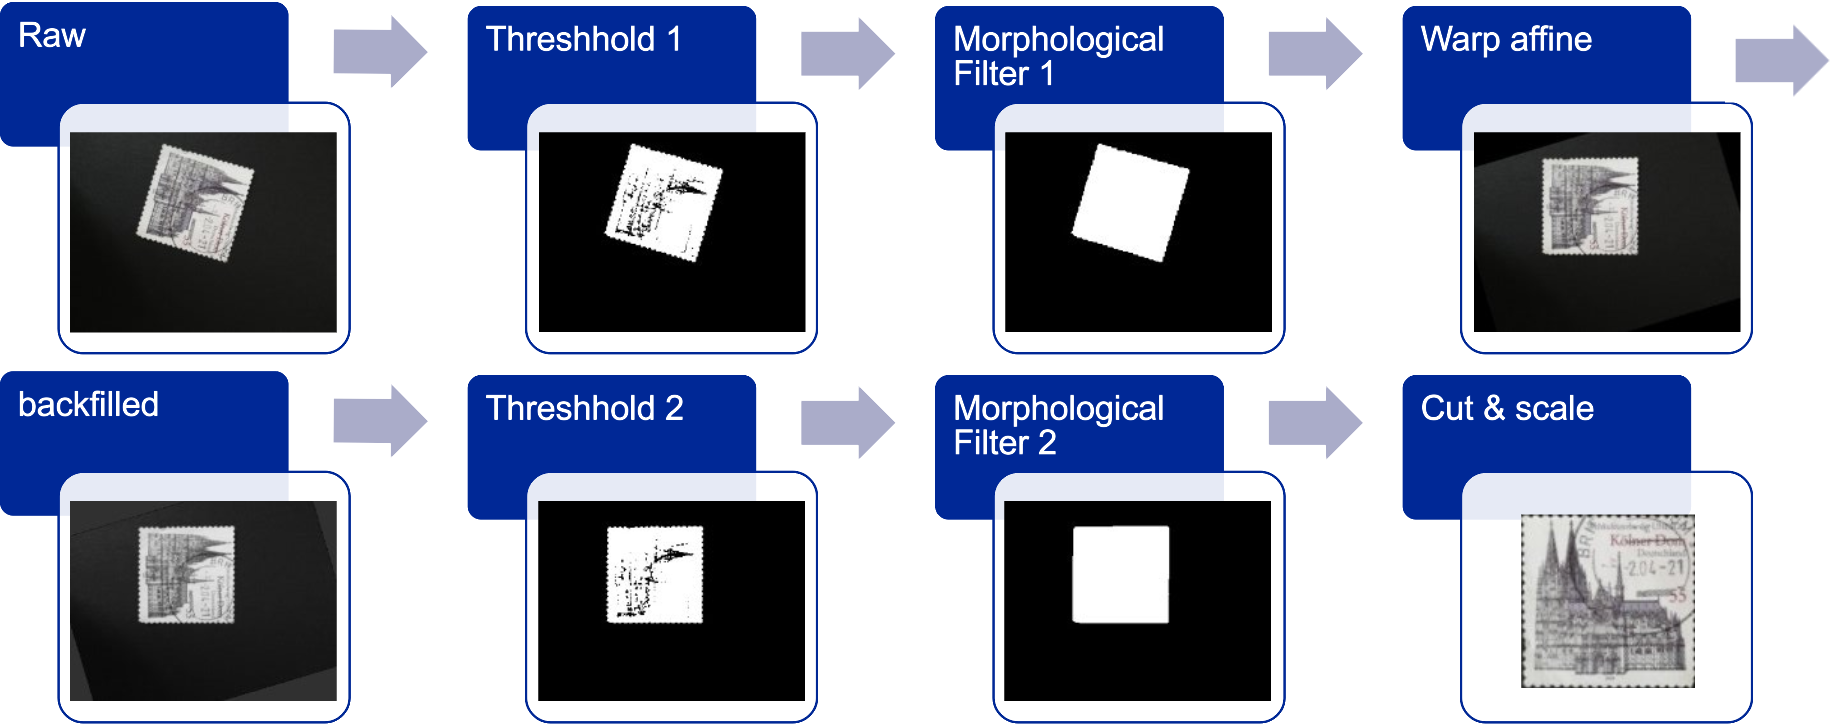
\includegraphics[width=\textwidth]{./bilder/bv_overview.png}
\caption{Übersicht über die Schritte der klassischen Bildverarbeitung}
\label{fig:bv_overview}
\end{figure}



\section{Beispiel ohne Komplikationen}
\label{sec_bv:paradebsp}

Im Folgenden wird der Ablauf der klassischen Bildverarbeitung an einem Beispiel, das ohne weiteren Aufwand funktioniert, genauer erläutert.
\begin{figure}

\begin{minipage}[t]{.75\linewidth}
Die beiden Bilder auf der rechten Seite sind Eingang und Ausgang des ersten Schrittes (Raw -> Threshold1). Das Raw Bild ist dabei ein RGB-Bild, auf dem die Briefmarke in zufälliger Orientierung zu sehen ist. Der Hintergrund ist matt und schwarz-grau. Der Übergang zu Threshold1 wird mit einer Otsu-Binarisierung bewerkstelligt. Es wird also in ein Graustufenbild übergegangen. Je nach Motiv der Briefmarke sind im Binärbild jedoch noch viele schwarze Stellen auf der Briefmarke. Dadurch resultiert die Marke nicht in einer einzelnen großen Kontur, sondern in vielen kleinen. Da wir jedoch erst mal das Bild gerade drehen wollen, bräuchten wir dafür eine einzige große, möglichst rechteckige Kontur.
\end{minipage}
\hfill
\begin{minipage}[t]{.2\linewidth}
  \strut\vspace*{-\baselineskip}\newline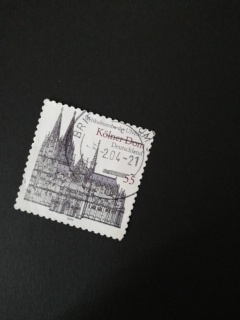
\includegraphics[width=\linewidth]{./bilder/start_dom}
  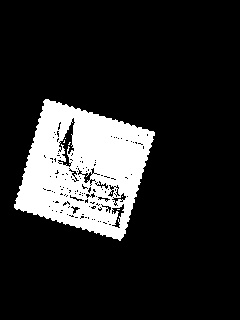
\includegraphics[width=\linewidth]{./bilder/bin1_dom}
  \caption{Übergang zu Threshold1}
  \label{fig:bv_th1}
\end{minipage}
\end{figure}
%%% ggf. weitere Abschnitte

\begin{figure}[h]
\begin{minipage}[t]{.75\linewidth}

Die Abbilung \ref{fig:bv_morph1} zeigt das Ergebnis des zweiten Schrittes der klassischen Bildverarbeitung. Hier sind keine dunklen Stellen mehr auf der Fläche der Briefmarke. Das wurde durch die Verwendung eines morphologischen Filters zur Erweiterung und Schließung von Konturen erreicht. Es wurde dafür eine quadratische Matrix mit Größe 11x11 verwendet. Bei einer Auflösung von 320x240 ist das ganz stattlich.
\end{minipage}
\hfill
\begin{minipage}[t]{.2\linewidth}
\strut\vspace*{-\baselineskip}
\newline
  
\includegraphics[width=\linewidth]{./bilder/bin1morph}
  \caption{Übergang zu morph. Filter1}
  \label{fig:bv_morph1}
\end{minipage}
\end{figure}

\begin{figure}[h]
\begin{minipage}[t]{.75\linewidth}

Die Abbildung \ref{fig:bv_rotimg} zeigt, wie gut die Kontur aus dem Binärbild nun die Briefmarke repräsentiert. Der blaue Rahmen aus dem oberen Teil der rechten Abbildung wird mit der opencv Methode minAreaRect aus der Kontur des Binärbildes gewonnen. Mit dem Verdrehwinkel dieses Rechtecks kann nun das ursprüngliche Bild ausgerichtet werden. Dies geschieht mithilfe der warpAffine Funktion. Um diese zu nutzen muss vorher noch eine 2D Rotationsmatrix erstellt werden. Dafür werden die Werte des Rechtecks verwendet. Das gerade gedrehte Bild ist im unteren Teil von Abbildung \ref{fig:bv_rotimg} zu erkenne.
\end{minipage}
\hfill
\begin{minipage}[t]{.2\linewidth}
  \strut\vspace*{-\baselineskip}\newline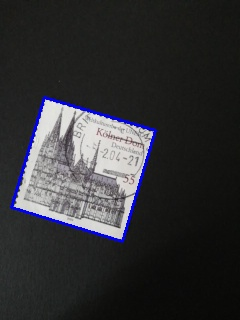
\includegraphics[width=\linewidth]{./bilder/minarearect_dom}
  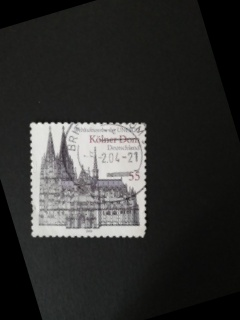
\includegraphics[width=\linewidth]{./bilder/rot_col}
  \caption{Rechteck, gerade gedrehtes Bild(warp Affine)}
  \label{fig:bv_rotimg}
\end{minipage}
\end{figure}

\begin{figure}[h]
\begin{minipage}[t]{.75\linewidth}

Aus dem gerade gedrehten Bild der Abbildung \ref{fig:bv_rotimg} kann nun wieder ein Binärbild erstellt werden. Wenn man darauf wieder morphologische Filter anwendet, kann ein Binärbild wie in Abbildung \ref{fig:bv_morph2} erreicht werden. Das Rechteck aus dieser Kontur ist nun geeignet, um die Briefmarke aus dem gerade gedrehten Farbbild auszuschneiden. Das ausgeschnittene Bildstück hat natürlich von Marke zu Marke andere Größenverhältnisse. Die Briefmarken haben schließlich nicht nur unterschiedliche Formate, sondern sind auch nicht alle aus der perfekt gleichen Distanz fotografiert worden. Da das NN eine bestimmte Inputgröße erfordert, muss hier also noch was geändert werden.
\end{minipage}
\hfill
\begin{minipage}[t]{.2\linewidth}
\strut\vspace*{-\baselineskip}
\newline
  
\includegraphics[width=\linewidth]{./bilder/bin2morph}
  \caption{Übergang zu morph. Filter2}
  \label{fig:bv_morph2}
\end{minipage}
\end{figure}


\section{Mögliche Probleme}
\label{sec_bv:probleme}
In diesem Abschnitt sollen aufgetretene Probleme geschildert und die dafür gefundenen Lösungen gezeigt werden.\\

\begin{figure}[h]
\begin{minipage}[t]{.75\linewidth}

Wie in der Abbildung \ref{fig:bv_prob1} zu sehen ist, können gerade gedrehte Bilder nach der Binarisierung durch ein ungünstiges Motiv mehrere zureichend große Konturen enthalten. Das Kriterium, das darüber entschieden hat, ob die Kontur eine potenzielle Briefmarke ist, war vorher nur die Fläche. Demnach würden hier drei Bilder für das NN ausgeschnitten werden. Um das zu verhindern, wird hier auf eine Hierarchiebedingung zurückgegriffen. Diese lautet, dass nur Konturen ohne Elternkontur weiter genutzt werden. Im Beispiel rechts fallen deshalb die blau und die rot markierten Konturen weg und nur die richtige, grüne, bleibt übrig.
\end{minipage}
\hfill
\begin{minipage}[t]{.2\linewidth}
\strut\vspace*{-\baselineskip}
\newline
  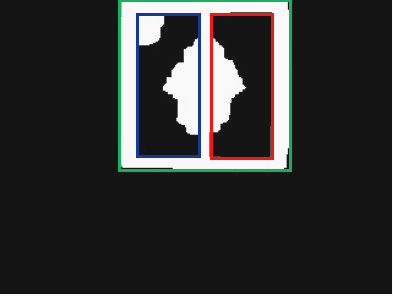
\includegraphics[width=\linewidth]{./bilder/prob1_bin}
  \caption{Binarisierung mit drei großen Konturen}
  \label{fig:bv_prob1}
\end{minipage}
\end{figure}

\begin{figure}[h]
\begin{minipage}[t]{.75\linewidth}

Ein weiteres Problem ist in Abbildung \ref{fig:bv_prob2} zu erkennen. Hier sind durch die Rotation große schwarze Flächen in den Ecken entstanden. Zur Binarisierung wird die Otsu-Methode verwendet, der Schwellwert zur Binarisierung wird also automatisch und abhängig vom Bild und dessen Histogramm festgelegt. Normalerweise ist der Hintergrund dunkler als die Briefmarke. Durch die dunklen Ecken wird aber eine dritten, noch dunklere Fläche eingeführt. Dadurch verschiebt sich der Schwellwert in eine mittlere Helligkeitsstufe und Teile des Hintergrundes werden mit Weiß binarisiert (oberer Teil der Abbildung). Um dieses Problem zu beheben wurden die dunklen Stellen mit dem Mittelwert der Helligkeit des Originalbildes nachgefärbt. Dadurch wird der Schwellwert deutlich schwächer beeinflusst und die Binarisieurng kann die Briefmarke wieder korrekt herausfiltern.
\end{minipage}
\hfill
\begin{minipage}[t]{.2\linewidth}
  \strut\vspace*{-\baselineskip}\newline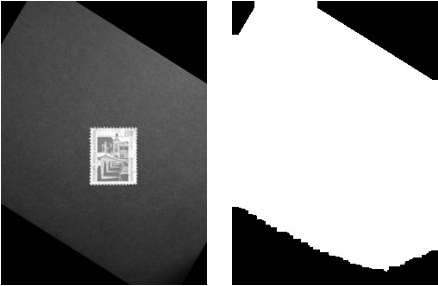
\includegraphics[width=\linewidth]{./bilder/prob2_bad_bin}
  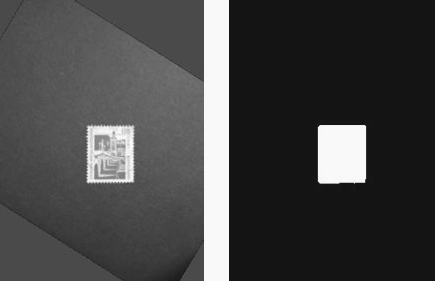
\includegraphics[width=\linewidth]{./bilder/prob2_good_bin}
  \caption{Binarisierungsproblem durch schwarze Ecken}
  \label{fig:bv_prob2}
\end{minipage}
\end{figure}


\begin{figure}[h]
\begin{minipage}[t]{.75\linewidth}

Das letzte Problem, das hier betrachtet werden soll, ist in Abbildung \ref{fig:bv_prob3} zu sehen. Auch wenn es mit dem menschlichen Auge nur schwer zu erkennen ist, ist das Bild sehr ungleichmäßig beleuchtet. Dadurch ist der ursprünglich schwarze Hintergrund in großen Bereichen sogar heller als die Briefmarke. Dadurch kann die Briefmarke gar nicht erst gerade gedreht werden. Im Vergleich zum vorher gegangenen Problem entstehen die Komplikationen also nicht erst durch während der Verarbeitung (wie zB. die schwarzen Ecken) sondern die Ursache dafür ist eine schlechte Qualität im Originalbild. Dieser Fall ist jedoch im ganzen Datensatz nur einmal aufgetreten.  Da wir entschieden haben, dass dieser Verlust verkraftbar ist, wurden hier keine weiteren Anstrengungen unternommen, um das letzte Bild auch noch zu retten.
\end{minipage}
\hfill
\begin{minipage}[t]{.2\linewidth}
  \strut\vspace*{-\baselineskip}\newline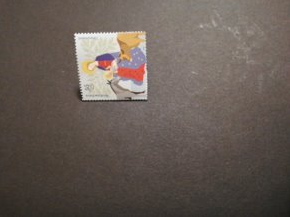
\includegraphics[width=\linewidth]{./bilder/prob3_pic}
  
\includegraphics[width=\linewidth]{./bilder/prob3_bad_bin}
  \caption{Binärisierungsproblem durch schlechte Lichtverhältnisse}
  \label{fig:bv_prob3}
\end{minipage}
\end{figure}

\section{Programmablaufplan}
\label{sec_bv:pap}
\begin{figure}[h]
\begin{minipage}[t]{.62\linewidth}
Der Programmablaufplan (PAP) zeigt, dass das Programm in zwei ineinander geschachtelten Schleifen abläuft. In der äußeren Schleife wird über die Liste der Bilder iteriert. Sollte eine Kontur mit ausreichender Größe durch die Binarisierung entstehen, wird daraufhin in die zweite Schleife übergegangen. In dieser wird über die gefundenen Konturen nach der zweiten Binarisierng und Dilatation iteriert. Zuerst wird dann die Fläche jeder Kontur abgefragt. Sollte die ausreichend sein, ist die nächste Bedingung die Hierarchiebedingung, die das Problem aus \ref{fig:bv_prob1} löst. Wenn beide Bedingungen erfüllt wurden wird der Bildausschnitt dem Benutzer angezeigt. Sollte dieser den Ausschnitt für gut befinden kann er mit der "g" Taste der Tastatur die Briefmarke abspeichern. Mit der "b" Taste werden diverse Zwischenergebnisse in Form von Bilddateien in einen separaten Ordner abgelegt. Dies erleichtert die Fehlersuche, ist aber für die Funktion des Programms unwichtig. Sollte das Bild weder gut noch einen interessanten Fehler hervorrufen, kann mit einer beliebigen Taste mit dem nächsten Bild fortgefahren werden. Zusätzlich zur Anzeige der Bilder gibt eine Konsolenausgabe auch noch Aufschluss über die Anzahl der Schleifendurchläufe (Anzahl bearbeiteter Bilder und Konturen). Durch die beiden Schleifen und das zweimalige Binarisieren ist der Code zwar nicht besonders performant, aber gut nachvollziehbar. Da für jede Marke eine Benutzereingabe erforderlich ist, ist es egal, dass der Code nicht besonders effizient programmiert wurde. Solange es dem Benutzer noch flüssig vorkommt, wird praktisch keine Zeit verloren, denn die Wartezeit auf die Eingabe macht die meiste Zeit aus.
\end{minipage}
\hfill
\begin{minipage}[t]{.33\linewidth}
\strut\vspace*{-\baselineskip}
\newline
  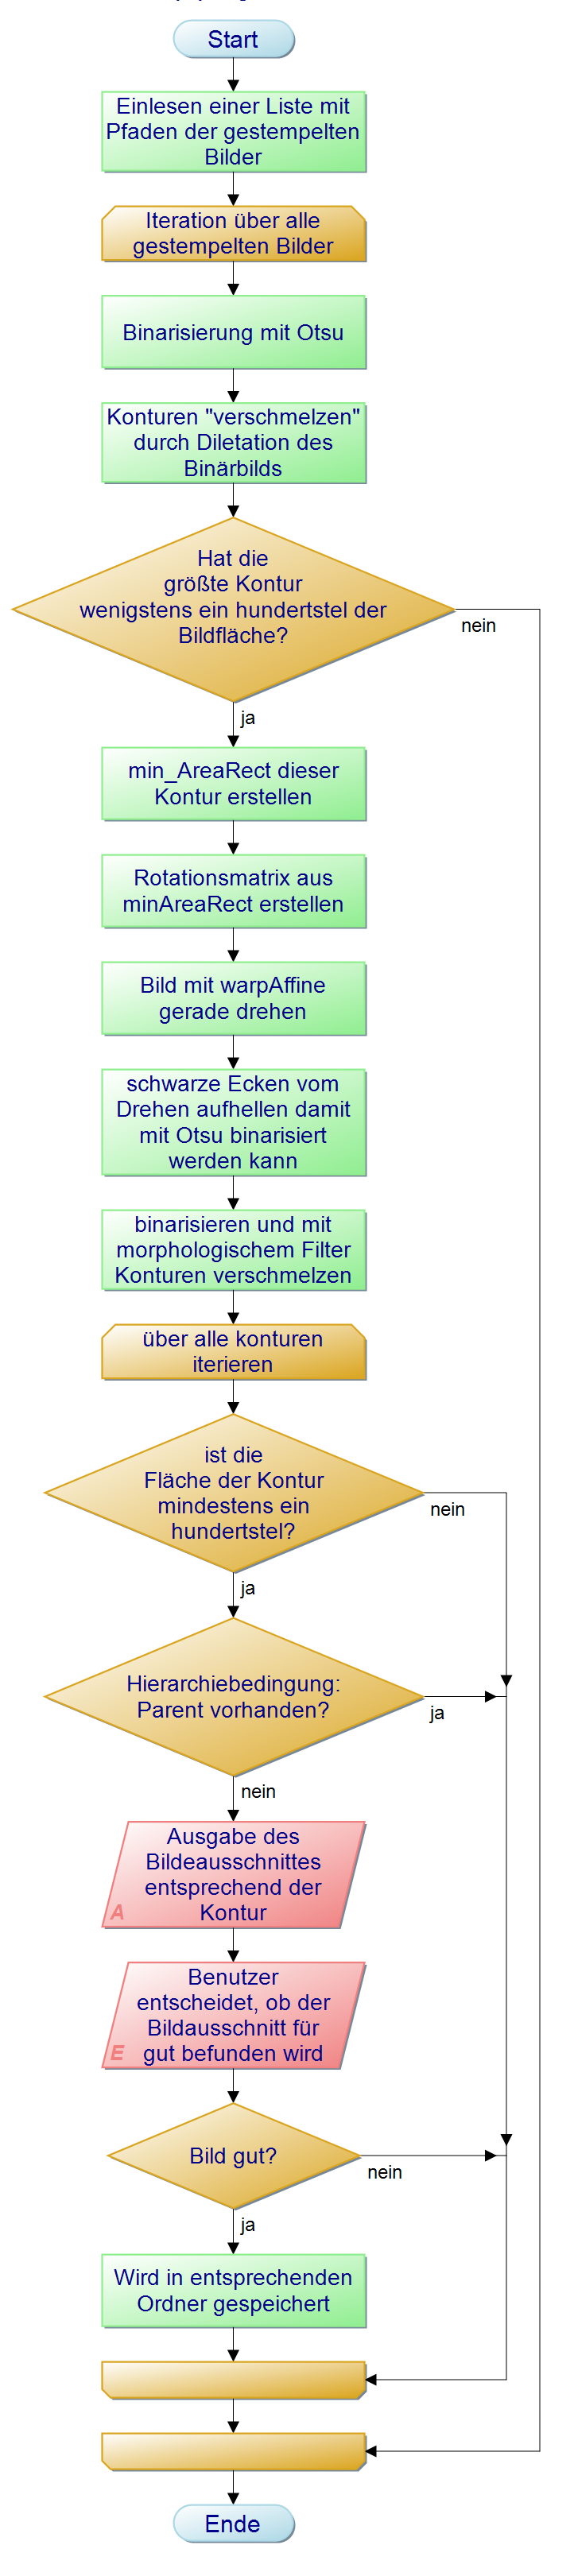
\includegraphics[width=\linewidth]{./bilder/BV_pap}
  \caption{Programmablaufplan Bildverarbeitung}
  \label{fig:bv_pap}
\end{minipage}
\end{figure}

\chapter{Neuronales Netzwerk} % (fold)
\label{sec:nn}
Für unsere Arbeit haben wir die Technik des \dq Transfer Learnig\dq\ angewandt. Dabei wird ein Netzwerk, dass ursprünglich auf eine andere, aber ähnliche Aufgabe trainiert wurde, wiederverwendet. Dafür muss meistens nur die Ausgabe angepasst werden. Deshalb müssen auch nur neu hinzugefügten Teile trainiert werden. Dadurch kann sehr viel Rechenaufwand gespart werden. Beim verwendeten NN handelt es sich um das MobileNetV2. Es kann für \dq Supervised Learning\dq\ Probleme zum Klassifizieren von Bildern verwendet werden.

\section{Architektur und Vorgehen}
\label{sec_nn:architecture}

Beim MobileNetV2 handelt es sich um ein \dq Convolutional Neuronal Network\dq\  (CNN). Diese werden hauptsächlich auf Bilder angewandt, haben aber auch noch andere Anwendungsgebiete. Ein CNN zeichnet sich durch die Schichten, in denen mithilfe von Matrizen durch Faltung unterschiedliche Merkmale der Bilder extrahiert werden, aus. Das MobileNetV2 wurde, wie der Name schon verrät, für die Anwendung auf mobilen Geräten entwickelt. Das bedeutet für Geräte mit niedriger Rechenleistung und ohne performante Grafikkarten wie Smartphones und Tablets.Es ist also eine sehr effektive Architektur nötig. Wie wird diese Effizienz nun aber erreicht? \\
Die Basis dieses NN ist eine \dq bottleneck depth-seperable convolution with residuals\dq\. \dq depth-seperable\dq\ bedeutet, dass nicht alle drei Farbkanäle auf einmal mit einem Tensor der Tiefe drei gefaltet werden, sondern alle Farbkanäle einzeln mit einem flachen Tensor gefaltet. Anschließend werden die Ergebnisse der drei einzelnen Operationen mit einer \dq Pointwise Convolution\dq\ verbunden. Dabei wird mit einem Tensor der Dimension 1x1x3 die Tiefe auf eins reduziert. Mit diesem Vorgehen verliert das Netzwerk, im Gegensatz zum direkten Anwenden eines Tensors der Tiefe drei, zwar Komplexität, aber die benötigten Rechnungen werden auch stark verringert. \cite{seperable_convolution} \\
\dq Residual Blocks\dq\ Verbinden den Eingang und den Ausgang eins Faltungsblocks mit einer Abkürzung. Durch die Addition dieser Zustände hat das NN Zugriff auf den Zustand vor der Faltung. Für gewöhnlich wird die Tiefe bei solchen Vorgängen immer erst reduziert und dann wieder erhöht. \cite{residuals_and_bottleneck} Beim MobileNetV2 wird das jedoch gedreht, da bei der \dq Depthwise Convolution\dq\ schon Parameter gespart wurden. Das \dq bottleneck\dq\ wird mit einer Relu6 Aktivierungsfunktion erreicht. Damit wird die Ausgabe auf einen Bereich von 0-6 limitiert. Diese Nichtlinearität wird in den \dq bottleneck depth-seperable convolution with residuals\dq\ jeweils nach einer Faltung eingefügt, abgesehen von der letzten \dq Pointwise Convolution\dq\ .


\begin{figure}[h]
\begin{minipage}[t]{.51\linewidth}

Die Abbildung \ref{fig:nn_arc} stellt eine \dq bottleneck depth-seperable convolution with residuals\dq\  Einheit dar. Sie besteht aus drei Faltungsoperationen(1x1, 3x3, 1x1), die die \dq Inverted Residuals\dq\ Struktur bilden. Insgesamt beinhaltet das Netzwerk nach einer ersten, reinen, Faltungsschicht 19 dieser Blöcke.
\end{minipage}
\hfill
\begin{minipage}[t]{.44\linewidth}
\strut\vspace*{-\baselineskip}
\newline
  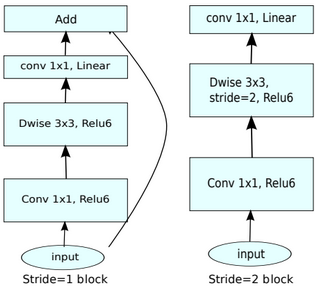
\includegraphics[width=\linewidth]{./bilder/mobnet_arc}
  \caption{Aufbau eines Blocks \cite{sandler2019mobilenetv2}}
  \label{fig:nn_arc}
\end{minipage}
\end{figure}

Dieses Netzwerk wurde von Google auf einen Datensatz von 1.4 Millionen Bilder aus 1000 Kategorien trainiert. Da sind gestempelte und nicht gestempelte Briefmarken natürlich nicht dabei. Jedoch werden auch um diese Kategorien zu differenzieren von NN zuerst Merkmalsextraktion betrieben. Durch das Nutzen eines anderen Outputlayers werden also aus den gleichen Merkmalen, die Google genutzt hat um 1000 Klassen zu unterscheiden, zwischen den zwei beiden Klassen unserer Projektarbeit unterschieden.
 


\section{Implementierung und Auswertung}
\label{sec_nn:impl}

\begin{figure}[h]
\begin{minipage}[t]{.71\linewidth}

Die Abbildung \ref{fig:nn_pap} zeigt, welche Schritte zur Implementierung in Python nötig waren. Zuerst ist natürlich wieder das Einlesen der Daten durchzuführen. Mit Hilfe einer assoziativen Liste (Dictionary) werden die Listen, die die Pfade zu den einzelnen Bildern enthalten, den beiden Klassen 0 und 1 zugewiesen. 0 steht in diesem Fall für gestempelt und 1 für ungestempelt. Als Nächstes wird der Datensatz zufällig durchgemischt und dann in Verhältnis eins zu drei aufgeteilt. Der dreiviertelste Teil wird nachher zum Training verwendet. Mit dem kleineren Teil wird die Auswertung des Ergebnisses durchgeführt. Danach werden die Farbwerte aller Kanäle durch 255 geteilt, um den Wertebereich auf 0-1 zu reduzieren. Abschließend werden die Bilder des Datensatzes auf die Größe 224x224 geändert. Das NN kann schließlich nur mit Bildern gleicher Größe arbeiten. Damit ist die Arbeit am Datensatz abgeschlossen. Als Nächstes muss das vortrainierte Model heruntergeladen werden. An diesem fehlt jedoch noch das Ausgabelayer. Das wird dann noch hinzugefügt. Damit ist das Netzwerk vollständig, nur die Gewichte des Ausgabelayers müssen noch trainiert werden. Das Training erfolgt über fünf Epochen mit dem Adam-Optimizer. Bereits nach diesen fünf Epochen konvergieren die Ergebnisse des NN sehr gut. Damit ist das NN dann bereit, die Bilder des Testdatensatzes zu klassifizieren. Dazu wird zu jedem Bild des Testdatensatzes ein Forwardpass durchgeführt. Hat die richtige Klasse den höheren Wert am Ausgabelayer, war die Klassifizierung erfolgreich. Über die Konsole wird der Benutzer dann informiert, wie das NN abgeschnitten hat. Zusätzlich werden die falsch klassifizierten Bilder dann dem Benutzer angezeigt. Damit kann er dann versuchen nachzuvollziehen, warum es falsch klassifiziert wurde.
\end{minipage}
\hfill
\begin{minipage}[t]{.24\linewidth}
\strut\vspace*{-\baselineskip}
\newline
  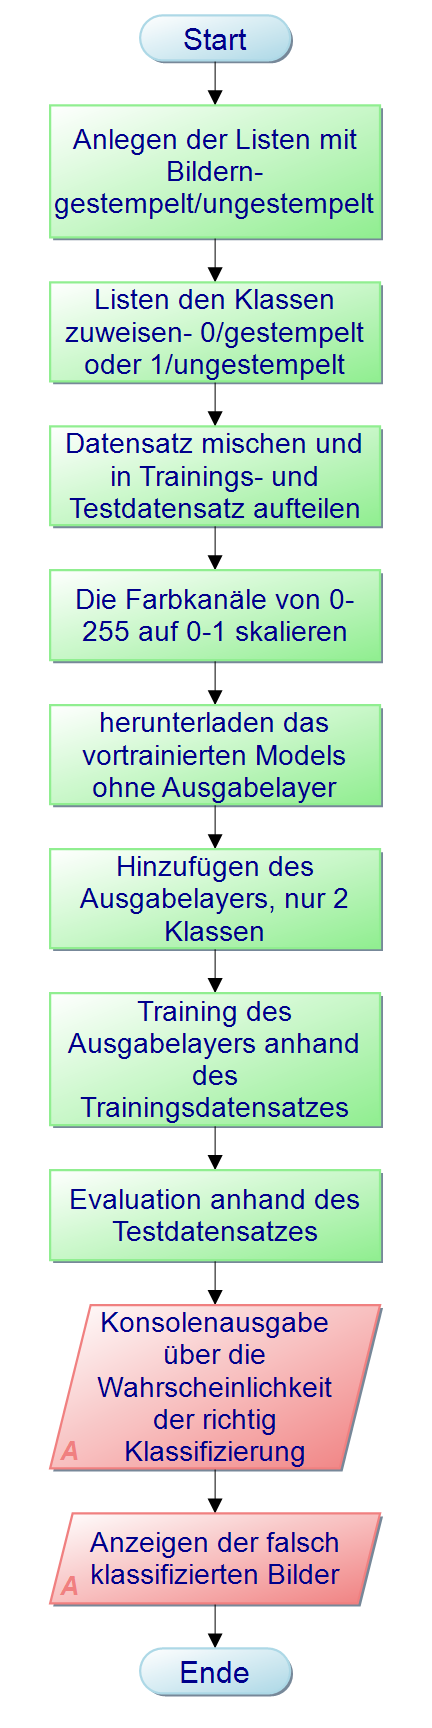
\includegraphics[width=\linewidth]{./bilder/Mobilenet}
  \caption{Programmablaufplan NN}
  \label{fig:nn_pap}
\end{minipage}
\end{figure}


\begin{figure}[h]
\begin{minipage}[t]{.48\linewidth}

Im Diagramm aus Abbildung \ref{fig:nn_pap} ist zu sehen, wie das NN in zehn Durchläufen abgeschnitten hat. Bei jedem Durchlauf wurden die Daten des Testdatensatzes und des Trainingsdatensatzes neu gemischt. Das Netzwerk wurde damit neu trainiert und evaluiert. Die Daten aus den zehn Durchgängen ergeben einen Mittelwert für die Klassifizierungsrate von 90,5\% und eine Standardabweichung von 3,5\%.  
\end{minipage}
\hfill
\begin{minipage}[t]{.47\linewidth}
\strut\vspace*{-\baselineskip}
\newline
  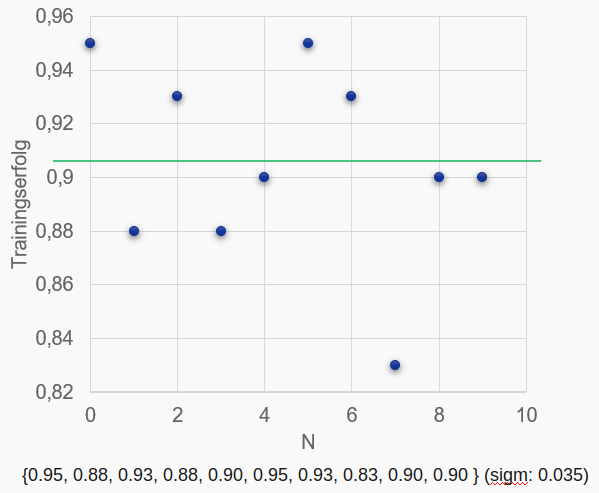
\includegraphics[width=\linewidth]{./bilder/auswertung}
  \caption{Auswertung von zehn Testläufen}
  \label{fig:nn_ausw}
\end{minipage}
\end{figure}

\chapter{Fazit} % (fold)
\label{sec:fazit}

Abschließend lässt sich sagen, dass das Projekt als Proof of Concept durchaus erfolgreich war. Es konnte gezeigt werden, dass mit dem NN MobilNetV2 mit einer zusätzlichen einfachen Vorverarbeitung Briefmarke in gestempelt und nicht gestempelt unterschieden werden können. Mit etwa 90\% ist die Rate an richtigen Klassifizierungen zwar nicht besonders hoch, doch angesichts des sowohl kleinen als auch qualitativ schlechten Datensatzes ist es kein schlechtes Ergebnis.\\
Eine Möglichkeit zum Verbessern des Datensatzes währe die Technik der \dq Data Augmentation\dq\ gewesen. Dabei werden aus den vorhandenen Daten weitere Daten durch Operationen wie Spiegelung, Drehung, Helligkeitsänderung etc. generiert und der Datensatz so erweitert.\\
Das Verbesserungspotenzial liegt jedoch nicht nur beim Datensatz, wenn auch das wahrscheinlich das größte Defizit unserer Arbeit ausmacht. Ein anderer Bereich, der wohl verbessert werden kann, ist die Auswahl des Netzwerkes. Hier hätte kein Fokus auf Effizienz gelegt werden müssen, denn durch das \dq Transfer Learning\dq\ ist der Trainingsbedarf sehr niedrig. 





% chapter fazit (end)

\appendix

\bibliography{literatur} 
\bibliographystyle{ieeetr}
\end{document}
